
% \chapter{GIỚI THIỆU VỀ CÔNG TY THỰC TẬP}
\begin{center}
	\section*{CHƯƠNG 1: GIỚI THIỆU}
\end{center}
\section{Giới thiệu chung}

\subsection{Giới thiệu về Công ty HPT}

Công ty Cổ phần Dịch vụ Công nghệ Tin học HPT (HPT Information Technology Services Joint Stock Company) được thành lập vào ngày 13/01/1995 và là một trong những doanh nghiệp tiên phong trong lĩnh vực công nghệ thông tin tại Việt Nam. Trải qua hơn ba thập kỷ hình thành và phát triển, HPT đã từng bước khẳng định vị thế của mình thông qua việc cung cấp các giải pháp công nghệ, dịch vụ chuyển đổi số và phát triển phần mềm cho nhiều doanh nghiệp, tổ chức trong và ngoài nước.

Với định hướng lấy công nghệ làm nền tảng phát triển, HPT luôn đầu tư vào nghiên cứu, đổi mới và ứng dụng các công nghệ hiện đại nhằm nâng cao chất lượng sản phẩm cũng như hiệu quả vận hành của khách hàng. Doanh nghiệp sở hữu đội ngũ kỹ sư, chuyên gia công nghệ có trình độ chuyên môn cao, cùng nhiều năm kinh nghiệm trong việc triển khai các dự án quy mô lớn thuộc nhiều lĩnh vực khác nhau như tài chính, ngân hàng, sản xuất, bán lẻ, giáo dục, y tế và cơ quan nhà nước.

Hiện nay, HPT cung cấp đa dạng các giải pháp và dịch vụ bao gồm:

\begin{itemize}
    \item Tư vấn và triển khai chuyển đổi số cho doanh nghiệp.
    \item Phát triển phần mềm theo yêu cầu (Software Development).
    \item Gia công phần mềm (Software Outsourcing).
    \item Tích hợp hệ thống (System Integration).
    \item Giải pháp điện toán đám mây (Cloud Computing).
    \item Giải pháp an toàn thông tin (Cyber Security).
    \item Quản trị hạ tầng CNTT và dịch vụ vận hành hệ thống.
\end{itemize}

Bên cạnh việc phát triển các giải pháp công nghệ, HPT còn chú trọng xây dựng quy trình phát triển phần mềm theo các tiêu chuẩn quốc tế như CMMI và ISO nhằm đảm bảo chất lượng sản phẩm, tối ưu quy trình làm việc và nâng cao hiệu quả triển khai dự án.

% \begin{figure}[H]
%     \centering
%     \includegraphics[width=0.7\textwidth]{include/image/hpt-building.jpg}
%     \caption{Trụ sở chính của Công ty Cổ phần Dịch vụ Công nghệ Tin học HPT}
%     \label{fig:hpt_building}
% \end{figure}

\subsection{Văn hóa doanh nghiệp}

Một trong những yếu tố góp phần tạo nên sự phát triển bền vững của HPT là văn hóa doanh nghiệp. Công ty luôn xây dựng môi trường làm việc chuyên nghiệp, cởi mở và khuyến khích tinh thần học hỏi, sáng tạo của mỗi cá nhân. Các nhân viên được tạo điều kiện phát triển kỹ năng chuyên môn, nâng cao năng lực làm việc nhóm và tiếp cận với các công nghệ mới.

HPT đề cao tinh thần trách nhiệm trong công việc, sự minh bạch trong giao tiếp cũng như khả năng hợp tác giữa các phòng ban. Mỗi dự án đều được triển khai theo quy trình rõ ràng với sự phối hợp chặt chẽ giữa các nhóm phân tích nghiệp vụ, phát triển phần mềm, kiểm thử và vận hành hệ thống nhằm đảm bảo tiến độ cũng như chất lượng sản phẩm.

Các giá trị cốt lõi mà HPT hướng tới bao gồm:

\begin{itemize}
    \item Chính trực và minh bạch.
    \item Cam kết với khách hàng.
    \item Chuyên nghiệp trong tác phong làm việc.
    \item Tinh thần đồng đội.
    \item Không ngừng đổi mới và sáng tạo.
\end{itemize}

Những giá trị này không chỉ góp phần xây dựng môi trường làm việc tích cực mà còn giúp HPT duy trì được uy tín với khách hàng trong quá trình phát triển lâu dài.

\subsection{Cơ cấu tổ chức}

HPT tổ chức hoạt động theo mô hình nhiều trung tâm chuyên môn nhằm đáp ứng yêu cầu của từng lĩnh vực công nghệ. Mỗi trung tâm đảm nhận một vai trò riêng nhưng luôn phối hợp chặt chẽ trong quá trình triển khai các dự án.

Các đơn vị chính của HPT bao gồm:

\begin{itemize}
    \item Trung tâm Giải pháp và Dịch vụ Phần mềm (HAS).
    \item Trung tâm Tích hợp Hệ thống (HSI).
    \item Trung tâm Dịch vụ Khách hàng (HSC).
    \item Trung tâm An toàn Thông tin (HSE).
    \item Trung tâm Giải pháp và Công nghệ Việt.
\end{itemize}

Ngoài trụ sở chính đặt tại Thành phố Hồ Chí Minh, HPT còn có các chi nhánh tại Hà Nội và Đà Nẵng nhằm mở rộng phạm vi hoạt động và hỗ trợ khách hàng trên toàn quốc.

Trong thời gian thực tập, em được phân công làm việc tại Chi nhánh Nguyễn Trường Tộ, Quận 4, Thành phố Hồ Chí Minh, thuộc Trung tâm Giải pháp và Dịch vụ Phần mềm (HAS). Tại đây, em có cơ hội tham gia vào dự án phát triển hệ thống quản lý thiết bị IoT cho máy lọc nước, đồng thời được tiếp cận với quy trình phát triển phần mềm, phân tích nghiệp vụ, thiết kế cơ sở dữ liệu và xây dựng các chức năng của hệ thống dưới sự hướng dẫn của các kỹ sư tại công ty.

\begin{figure}[H]
    \centering
    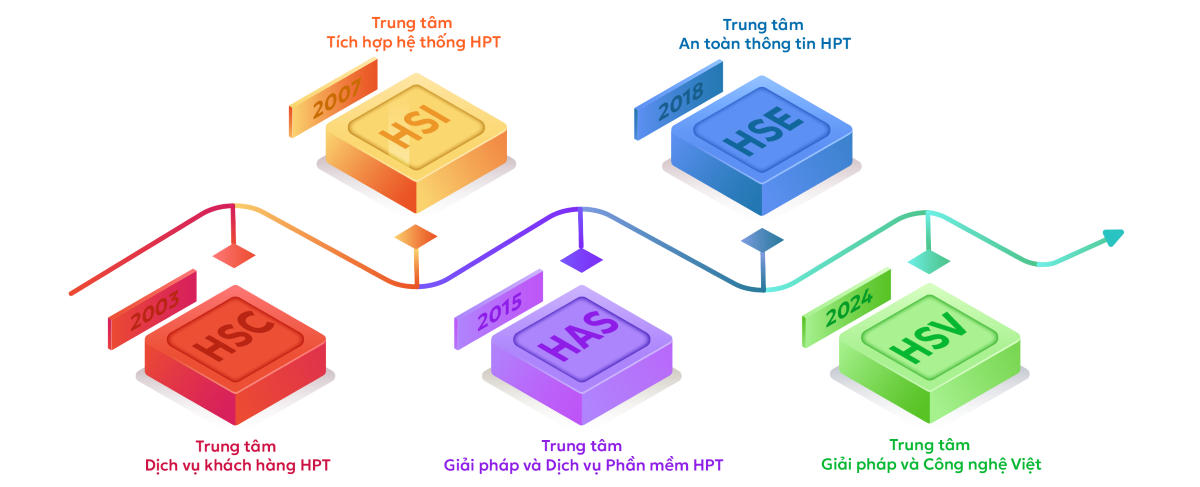
\includegraphics[width=0.85\textwidth]{include/image/5TT.png}
    \caption{Sơ đồ tổ chức của Công ty Cổ phần Dịch vụ Công nghệ Tin học HPT}
    \label{fig:hpt_org}
\end{figure}

\subsection{Giới thiệu về nội dung thực tập}


\begin{table}[H]
\centering
\renewcommand{\arraystretch}{1.4}
\begin{tabularx}{\textwidth}{|c|X|}
\hline
\textbf{Tuần} & \centering\arraybackslash\textbf{Nội dung công việc} \\ \hline

1 &
Giới thiệu doanh nghiệp, môi trường làm việc, quy trình phát triển sản phẩm và định hướng thực tập.
\\ \hline

2 &
Tìm hiểu hệ thống hiện tại, kiến trúc giải pháp, quy trình nghiệp vụ và mô hình IoT của dự án.
\\ \hline

3 &
Tìm hiểu nghiệp vụ hệ thống, làm quen với Web Backend, khảo sát kiến trúc dữ liệu và luồng xử lý của hệ thống.
\\ \hline

4 &
Khảo sát phần cứng máy lọc nước, phân tích bo mạch điều khiển, cảm biến và khả năng tích hợp IoT; nghiên cứu phương án thu thập dữ liệu từ thiết bị.
\\ \hline

5 &
Kết nối thiết bị với MQTT Broker, xây dựng cơ chế publish dữ liệu từ thiết bị lên hệ thống.
\\ \hline

6 &
Xây dựng chức năng thu thập, xử lý và lưu trữ dữ liệu từ máy lọc nước; phát triển dashboard giám sát thiết bị theo thời gian thực.
\\ \hline

7 &
Kiểm thử hệ thống, tối ưu và hoàn thiện các chức năng được giao.
\\ \hline

8 &
Tổng kết, hoàn thiện tài liệu và báo cáo.
\\ \hline

\end{tabularx}
\caption{Kế hoạch thực tập theo từng tuần}
\label{tab:internship_plan}
\end{table}

\href{https://drive.google.com/drive/folders/1DUJnd1QZbqKCEJuZf9zSlL2L1OZpgIk4?usp=sharing}{Tài liệu thực tập}
https://drive.google.com/drive/folders/1DUJnd1QZbqKCEJuZf9zSlL2L1OZpgIk4?usp=sharing